\documentclass[tikz,border=4pt]{standalone}
\usepackage{tikz}\usetikzlibrary{arrows.meta,positioning}
\definecolor{nebula}{HTML}{6366F1}\definecolor{spark}{HTML}{14B8A6}
\begin{document}
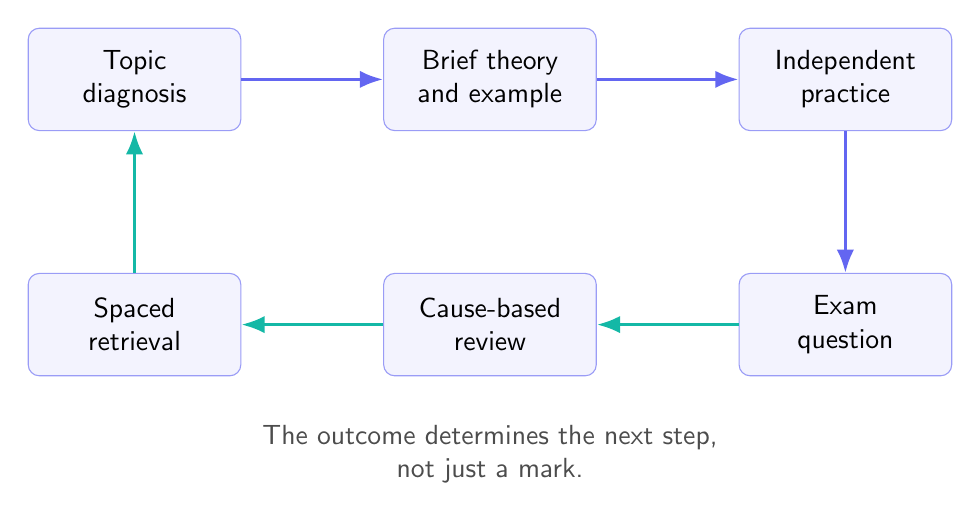
\begin{tikzpicture}[font=\sffamily,>=Latex,node distance=18mm]
  \tikzset{stage/.style={rounded corners=4pt,draw=nebula!65,fill=nebula!8,minimum width=27mm,minimum height=13mm,align=center}}
  \node[stage] (d) {Topic\\diagnosis}; \node[stage,right=of d] (t) {Brief theory\\and example}; \node[stage,right=of t] (p) {Independent\\practice};
  \node[stage,below=of p] (e) {Exam\\question}; \node[stage,left=of e] (c) {Cause-based\\review}; \node[stage,left=of c] (r) {Spaced\\retrieval};
  \draw[->,very thick,nebula] (d)--(t); \draw[->,very thick,nebula] (t)--(p); \draw[->,very thick,nebula] (p)--(e); \draw[->,very thick,spark] (e)--(c); \draw[->,very thick,spark] (c)--(r); \draw[->,very thick,spark] (r)--(d);
  \node[below=5mm of c,align=center,text=black!70] {The outcome determines the next step,\\not just a mark.};
\end{tikzpicture}
\end{document}
